
Information is incredibly important in programming,
whether it is what a command does, how its used,
or what is contained in variables.
I take information as a starting point,
and this section is all about obtaining and storing various forms of information.


\subsection{The \texttt{help} command}

Perhaps the most important command in Stata,
\texttt{help} allows quick access to information on \emph{any} command Stata has.
The help-files Stata provides are incredibly detailed,
including information on how to use the command (its \emph{syntax}),
what the command does, its output, examples,
and sometimes even the theory behind it.
As useful as it is, the help-files might seem daunting at first.
Understanding their structure is key to (quickly) obtain information without falling into despair.
I'll highlight what I believe to be the most important parts of the help-files through an example.

If I type \mintinline{stata}{help summarize},
Stata opens the window in \cref{fig:hlpsum}.
In help-files, the typography on its own already gives us a lot of information.

\textbf{Bold} words indicate commands or options; if we want to use these,
we type them exactly as they are written down.
In our case,
\textbf{\texttt{summarize}} is written in bold under the syntax heading.
It is, as we know, indeed a command.

\textit{Italicised} text indicates something that should be substituted.
Here, \textit{\texttt{varlist}} tells us that we should write down a list of variable names here -- should we want to use this option.

Optional arguments and functions are indicated by being [in brackets].
This means that anything that is written within brackets in the syntax is something that does not have to be specified for a command to work.

\underline{Underlined} text indicates the \emph{minimum} abbreviation of a command or option.
In the case of \mintinline{stata}{summarize},
I could simply write \mintinline{stata}{su}.
Additional letters are also allowed and how to use this is mostly personal preference.
Personally, I always write \mintinline{stata}{sum} as its clearer to me what that means than \mintinline{stata}{su} would,
but it still saves me the time and space from writing the command out in its entirety.
When abbreviating commands,
make sure you are familiar enough with them to remember what an abbreviation means if you open your do-files one week later.
Having to look it up every time you see an abbreviation can be quite a pain.

Finally, any text in blue is a hyperlink,
generally leading to more information on whatever is written down.\footnote{~Note that the exact colour depends on Stata's colour scheme, but the default and dark schemes do use blue.}

\begin{figure}[tbp]\centering
  \caption{Help-file for \texttt{summarize}}\label{fig:hlpsum}
  \vspace{1ex}
  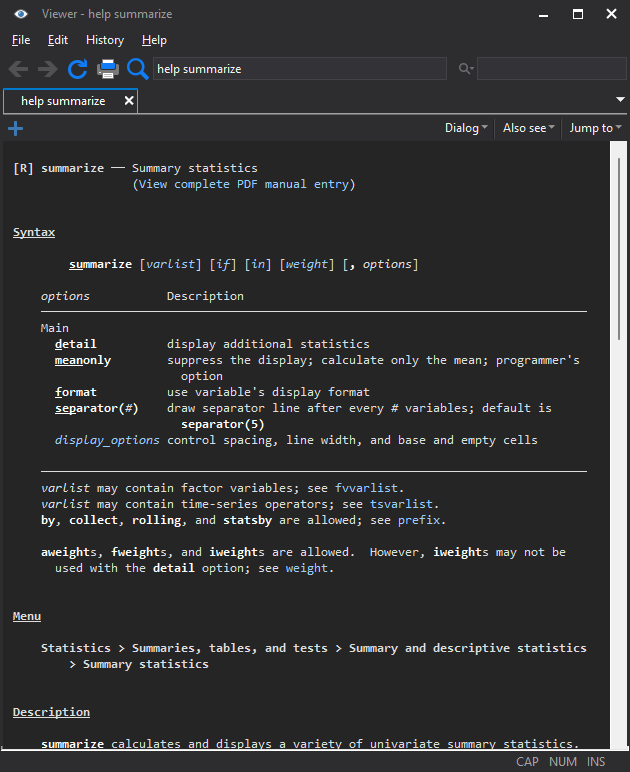
\includegraphics[width=0.85\textwidth]{helpsummarize}
\end{figure}

\subsection{scalars and matrices}

storing information in scalars and matrices

\subsection{display}

display command

\subsection{macros}

globals and locals
